\documentclass{article}

\usepackage{tikz}
\usepackage[margin=1in]{geometry}
\usepackage{mathtools}

\usepackage{amsmath}
\usepackage{cancel}
\usepackage{pdfpages}

\usepackage{listings}
\renewcommand{\tt}[1]{\texttt{#1}}
%\newcommand{\linux}[1]{\begin{lstlisting}[language=bash] #1 \end{lstlisting}}
\lstnewenvironment{linux}{\lstset{language=bash}}{}

\renewcommand{\c}[1]{\cancel{#1}}
\begin{document}
\begin{center}
\Large{MA/CSSE Homework 8}\\
Due 5/19
\end{center}
\vspace{.25in}
\noindent{\textbf{Directions}}\\
  \begin{itemize}
   \item \textbf{Each problem must be self-contained in a file}, named
     properly, and \textbf{must compile using the
      command} \texttt{mpicc filename.c}\\

  \item Turn in each \tt{.c} file to the dropbox. \textbf{Do not
      create a \tt{.zip} file}

  \end{itemize}


\section*{Problems}

\noindent{\textbf{Level:}Easy}\\
\begin{enumerate}
\item The \textit{Sieve of Eratosthenes} is a classic method for
  determining all the prime numbers between $2$ and $k$.  It, and its variants, are
  still reasonable methods for finding moderately sized prime numbers
  today.  

  The sieving method works by striking out multiples of all known
  prime numbers.  We start with a list, $L$ that contains all integers
  2 through $k$.  
\[L=\{2,3,4,5,6,7,8,9,10,11,12,13,14,15,16,17,\dots,k\}\]
2 is the smallest number in the list, so we take it as prime.  We now
walk through the list in steps of 2, marking off all the multiples of
2. 
\[L=\left\{\boxed{2},3,\c{4},5,\c{6},7,\c{8},9,\c{10},11,\c{12},13,\c{14},15,\c{16},17,\dots,k\right\}.\]
The next smallest unmarked integer in the list is 3, which we now
know is prime. We mark $3$ as prime and strike out all the multiples
of 3. 
\[L=\left\{\boxed{2},\boxed{3},\c{4},5,\c{6},7,\c{8},\c{9},\c{10},11,\c{12},13,\c{14},\c{15},\c{16},17,\dots,k\right\}.\]
The next smallest entry in the list is 5, which we mark as prime, and
strike out all multiples of 5. 
\[L=\left\{\boxed{2},\boxed{3},\c{4},\boxed{5},\c{6},7,\c{8},\c{9},\c{10},11,\c{12},13,\c{14},\c{15},\c{16},17,\dots,k\right\}.\]
This process is repeated until we have marked out all the multiples of
$j\le\sqrt{k}$. At that point all unmarked entries in $L$ may be
safely marked as prime. 

We may think of the sieving method as a sequence of filters that are
applied to $L$.  First is the filter that discards all multiples of
2.  The first element to survive that filter is 3, and so we run a
filter that discards all multiples of 3 on the output of the first
filter. 

A pipelined version of this algorithm might work as follows: Processor
0 acts as a list-generator and $2-$filter.  It checks every number $x$
between $0$ and $k$ to see if $x$ is a multiple of 2. Every number
that is not a multiple of two is passed to the next processor.
Processor 1 first receives 3 from rank 0, and so becomes a
$3-$filter.  Processor $2$ becomes a $5-$filter, processor $3$ a $7-$
filter, processor $4$ a $11-$filter, and so on. See the figure below:

\begin{center}
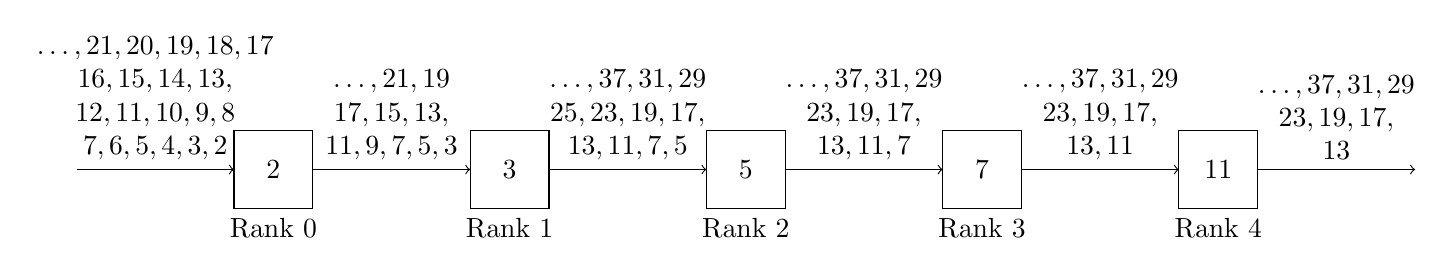
\begin{tikzpicture}
\draw [->](-2,0.5) -- (0,0.5);
\draw (0,0) rectangle (1,1);
\draw [->] (1,0.5) -- (3,0.5);
\draw (3,0) rectangle (4,1);
\draw [->] (4,0.5) -- (6,0.5);
\draw (6,0) rectangle (7,1);
\draw [->] (7,0.5) -- (9,0.5);
\draw (9,0) rectangle (10,1);
\draw [->] (10,0.5) -- (12,0.5);
\draw (12,0) rectangle (13,1);
\draw [->] (13,0.5) -- (15,0.5);
\node [below] at (0.5,0) {Rank 0};
\node [below] at (3.5,0) {Rank 1};
\node [below] at (6.5,0) {Rank 2};
\node [below] at (9.5,0) {Rank 3};
\node [below] at (12.5,0) {Rank 4};
\node at (0.5,0.5) {2};
\node at (3.5,0.5) {3};
\node at (6.5,0.5) {5};
\node at (9.5,0.5) {7};
\node at (12.5,0.5) {11};
\node [align=center,above] at (-1,0.5) {$\dots,21,20,19,18,17$\\$16,15,14,13,$\\$12,11,10,9,8$\\$7,6,5,4,3,2$};
\node [align=center,above] at (2,0.5) {$\dots,21,19$\\$17,15,13,$\\$11,9,7,5,3$};
\node [align=center,above] at (5,0.5) {$\dots,37,31,29$\\$25,23,19,17,$\\$13,11,7,5$};
\node [align=center,above] at (8,0.5) {$\dots,37,31,29$\\$23,19,17,$\\$13,11,7$};
\node [align=center,above] at (11,0.5) {$\dots,37,31,29$\\$23,19,17,$\\$13,11$};
\node [align=center,above] at (14,0.5) {$\dots,37,31,29$\\$23,19,17,$\\$13$};
\end{tikzpicture}
\end{center}
We can see that all the "filters" are prime numbers, and that any
number exiting rank 4 is not divisible by $2,3,5,7,$ or $11$.  Thus,
any number making it past rank 4 that is less than $121$ must be
prime. 

This is an effecitive method to determine the list of primes that are
less than $p^2$, where $p$ is the number of processors available.  To
allow us to generate bigger lists, we can have each processor be a
filter for $N/p$ primes, rather than just for 1 prime.  See the
figure. 

\begin{center}
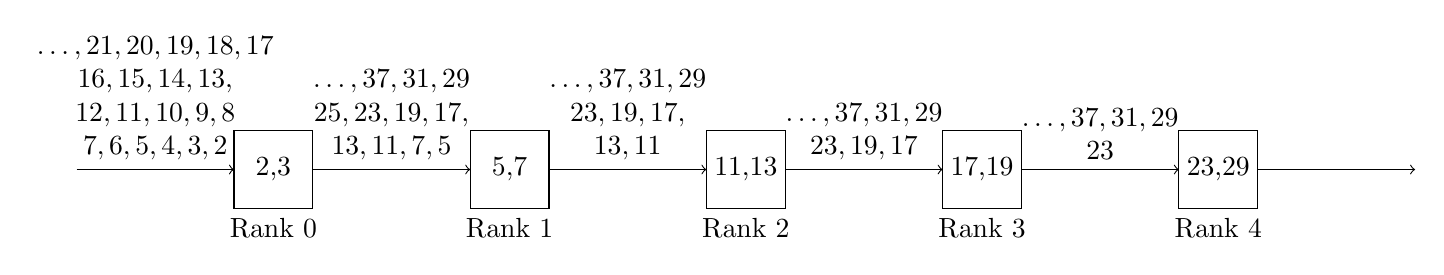
\begin{tikzpicture}
\draw [->](-2,0.5) -- (0,0.5);
\draw (0,0) rectangle (1,1);
\draw [->] (1,0.5) -- (3,0.5);
\draw (3,0) rectangle (4,1);
\draw [->] (4,0.5) -- (6,0.5);
\draw (6,0) rectangle (7,1);
\draw [->] (7,0.5) -- (9,0.5);
\draw (9,0) rectangle (10,1);
\draw [->] (10,0.5) -- (12,0.5);
\draw (12,0) rectangle (13,1);
\draw [->] (13,0.5) -- (15,0.5);
\node [below] at (0.5,0) {Rank 0};
\node [below] at (3.5,0) {Rank 1};
\node [below] at (6.5,0) {Rank 2};
\node [below] at (9.5,0) {Rank 3};
\node [below] at (12.5,0) {Rank 4};
\node at (0.5,0.5) {2,3};
\node at (3.5,0.5) {5,7};
\node at (6.5,0.5) {11,13};
\node at (9.5,0.5) {17,19};
\node at (12.5,0.5) {23,29};
\node [align=center,above] at (-1,0.5) {$\dots,21,20,19,18,17$\\$16,15,14,13,$\\$12,11,10,9,8$\\$7,6,5,4,3,2$};
\node [align=center,above] at (2,0.5) {$\dots,37,31,29$\\$25,23,19,17,$\\$13,11,7,5$};
\node [align=center,above] at (5,0.5){$\dots,37,31,29$\\$23,19,17,$\\$13,11$};
\node [align=center,above] at (8,0.5) {$\dots,37,31,29$\\$23,19,17$};
\node [align=center,above] at (11,0.5) {$\dots,37,31,29$\\$23$};
\end{tikzpicture}
\end{center}

Write a program in \tt{eratosthenes.c} that calculates the first $N$
primes using the Sieve of Eratosthenes.  Each processor should act as
a filter for at most $\ceil{N/p}+1$ primes. 

Note that rank 0 does not know ahead of time how many number to put
into the pipeline, that must be detected as we go.  Rank $p$ is the
only processor than can detect when we have generated $N$ primes.
When the $N^{th}$ prime is found, have rank $p$ send a special message
to rank 0, telling it to stop processing. When rank 0 stop processing,
have it send a message to rank 1, then from rank 1 to 2, and so on. 

Rank 0 must periodically check to see if a message has arrived from
rank $p$, telling rank 0 to stop processing.  Use the command \\
\\
\tt{int MPI\_Iprobe(int source, int tag, MPI\_Comm comm, int *flag,
  MPI\_Status *status)}\\
\\
on the root to check to see if there is a message from rank $p$.  \tt{MPI\_Iprobe}
checks to see if there is a message from \tt{source} with the given
\tt{tag} on the communicator \tt{comm}.  If there is, then \tt{flag}
is set to true and the \tt{status} variable is filled up with all the
standard information about the message.  For instance, you could check
to see how large the message is, before receiving it.  If there is no
message available that matches the criteria, \tt{flag} is set to
false.  In either case \\tt{MPI\_Iprobe} \textbf{will not block},
which makes it perfect for this use case. 
  
Once the first $N$ primes are found,use \tt{MPI\_Gatherv} to send them
all back to the master process, and have the root print them if
requested, and write a file if requested. 

The standard implementation may be compiled with \\
\tt{\$ mpicc objs/eratosthenes\_standard.<arch>.o -o eratosthenes\_standard}

The file \tt{eratosthenes\_start.c} and \tt{eratosthenes\_helpers.h}
give you some framework. 

In addition to passing \tt{test\_eratosthenes.py}, hand in a file that
contains the first $10^6$ prime numbers named \tt{lots\_o\_primes.txt}. 


\end{enumerate}

\newpage

\noindent{\textbf{Level:} Difficult}

\begin{enumerate}
\item Create a program in \tt{linear\_solve.c} that uses the pipelined
  method of Chapter 11 (p355) with striped partitioning to solve
  linear systems of equations.  

In particular, suppose we want to solve a linear system of equations,
$Ax=b$.  Partition $A$ and $b$ so that each processor is responsible
for roughly $n/p$ contiguous rows of $A$ and the same roughly $n/p$
rows of $b$.  Rank 0 begins the algorithm by passing row 0 of $A$ and
$b$ to rank 1. Rank 1 forwards Row 0 to rank 2, which forward to rank
3, and so on.  Once each processor, $j$,  has forwarded row 0 to rank
$j+1$, rank $j$ performs elimination in column 0 on the rows for which
it is responsible.  

Once rank 0 is done with elimination in column 0, it forwards row 1 to
processor 1, and then begins elimination in column 1.  The method
continues until the matrix is in row-echelon form.  Once the matrix is
in row-echelon form, use back substitution, also pipelined, to find
the solution vector $x$.   Collect $x$ on the root node, produce an
output file or print $x$ out if requested.  See the attached pages for
another description. 

The standard code may be compiled with\\
\tt{\$ mpicc objs/linear\_solve\_standard.<arch>.o -o
  linear\_solve\_standard}\\

You need to respect the options provided in the \tt{options}
structure, the file \tt{linear\_solve\_start.c} provides a good
framework.  

The root node should be the only matrix that reads in $A$ and $b$. You
should use \tt{MPI\_Scatterv} to distribute the proper partitions of
$A$ and $b$ to the other nodes. There is no need to call a collective
operation to gather $x$ -- back substitution will naturally lead to
rank 0 having a full copy of $x$. 

The function \tt{residual} calculates $\sum_i
\left|(Ax)_i-b_i\right|$.  You can use it to check to see if you have
computed the correct solution.  If \tt{residual(A,x,b)} is very small
(like $10^{-10}$) then $x$ is very very close to the actual solution to
$Ax=b$.  

You may assume that $A$ is non-singular, and that pivoting is not
needed in order to get a good solution to $Ax=b$.  You can generate
random matrices for testing your code with \tt{rand\_inv\_matrix n}
and you can generate a random matrix (good for making $b$) with
\tt{rand\_matrix m n}. 

Note that, with the exception of the initial \tt{Scatterv}, each rank $j$
only needs to communicate with rank $j-1$ during elimination, and with
rank $j+1$ during back substitution.  Your code must produce the
correct results, respect all command line options, and must run within
$2x$ time of the standard code. 

\noindent\textbf{A note on sending rows:} The matrix data structure
is storing rows contiguously.  So, if you want to send rows 3 and 4 of
matrix $A$, and matrix $A$ is 20 wide, you can use just one
\tt{MPI\_Send} like this\\
\tt{MPI\_Send(A.data[3],40,MPI\_DOUBLE,...)}
 
\end{enumerate}

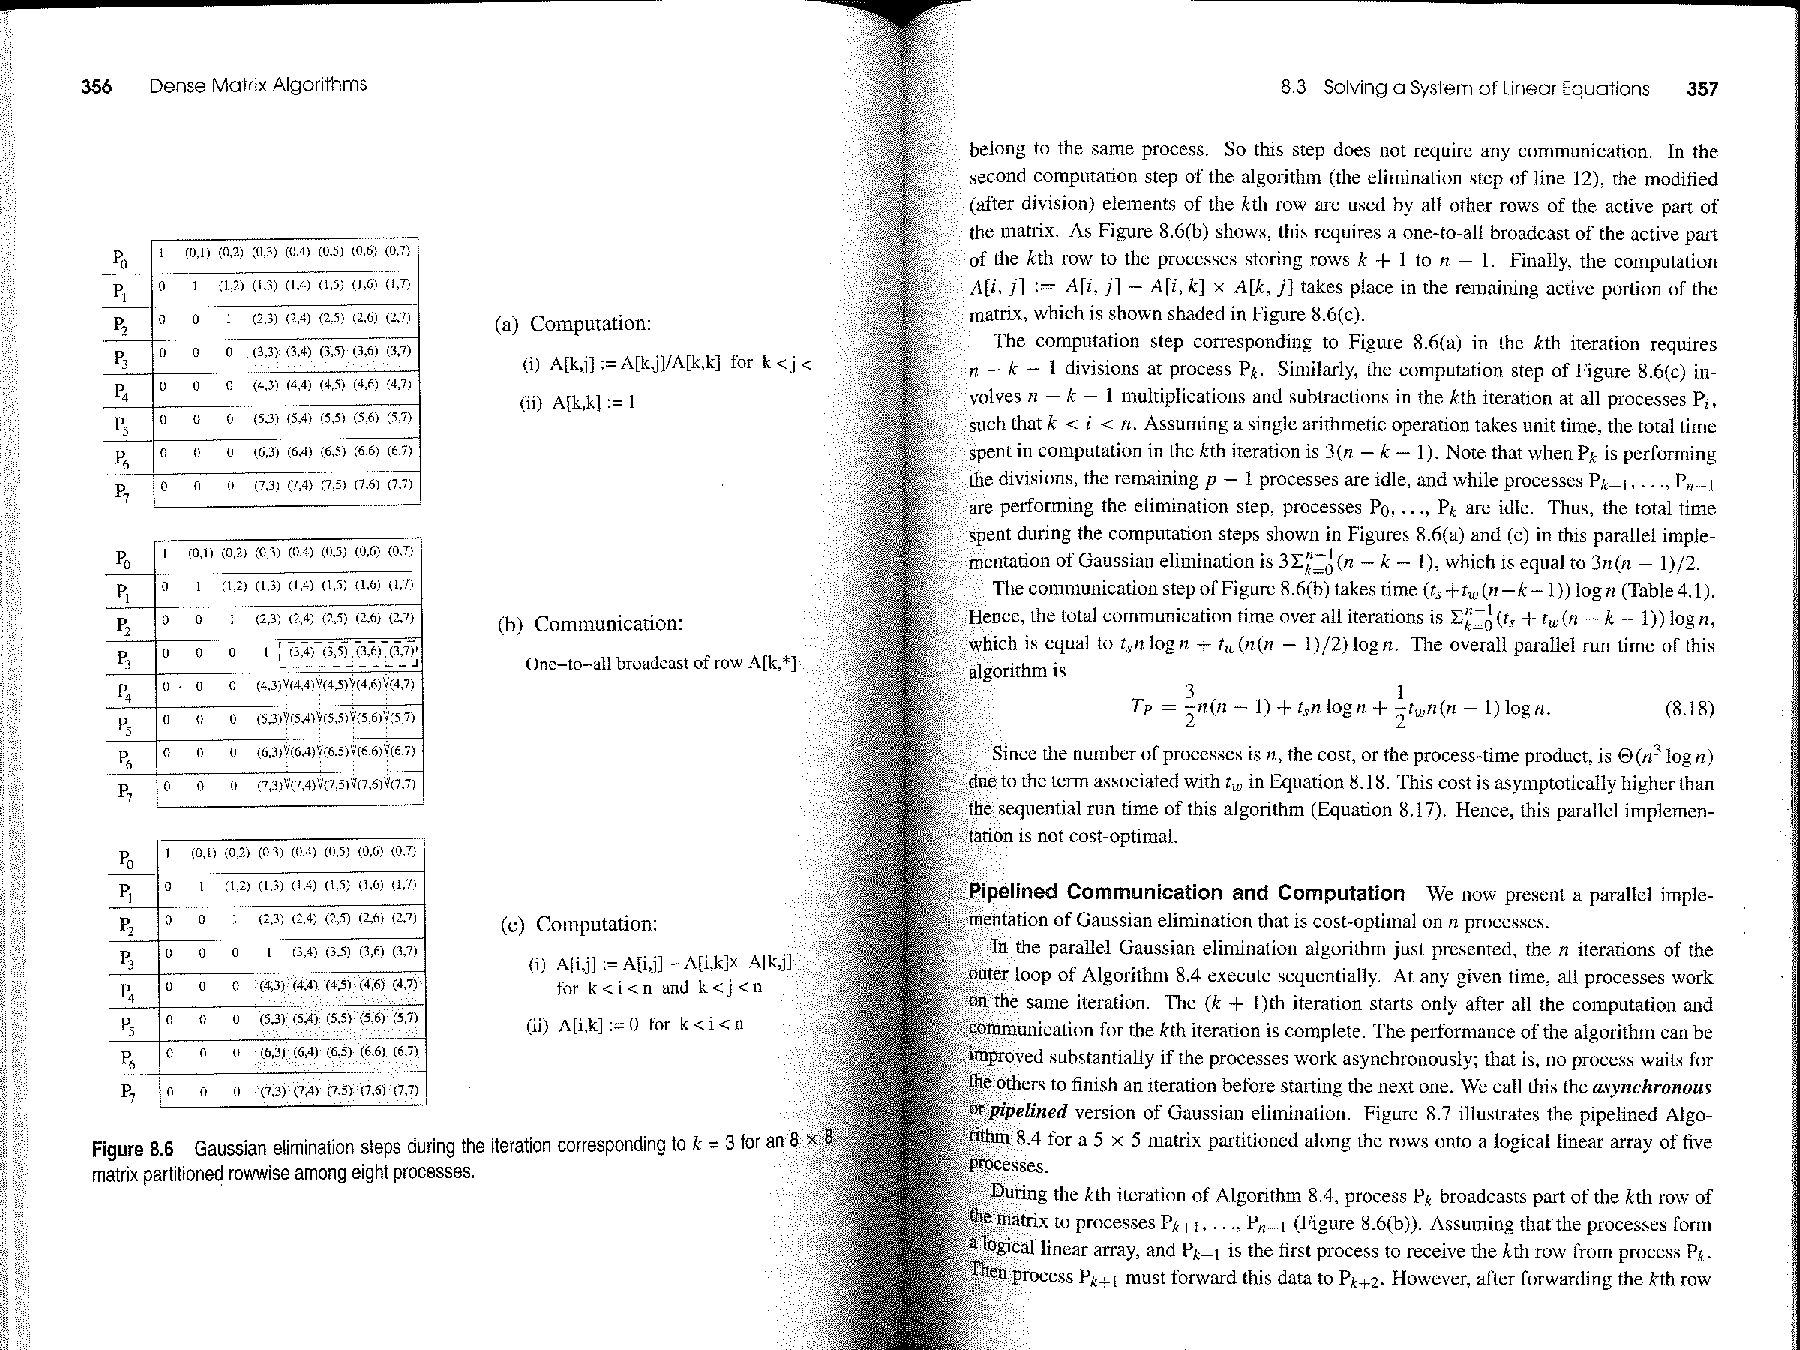
\includepdf[pages=-]{scans.pdf}



\end{document}
